\documentclass[../borwein-lewis_notes.tex]{subfiles}
\begin{document}
\maketitle
\subsection{2.3 Max-functions}
First order necessary conditions for an optimization problem with 
constraints involving differentiable functions will be obtained by 
considering the \textit{max-function}
\begin{equation}
\label{2.3.1}
g(x) = \max_{i=0,1,\ldots, m} g_i(x).
\end{equation}
\begin{proposition}[2.3.2 (Directional derivatives of max-functions)]
Let $\bar x\in\inter C\subset\E$. Suppose $g_0,\ldots, g_m:C\to\R$ 
are continuous and differentiable at $\bar x$. Furthermore, denote 
$K=\{i\mid g_i(\bar x) = g(\bar x)\}$. Then for all directions 
$d\in\E$, the directional derivative of the max-function $g$ 
in \eqref{2.3.1} is
\label{2.3.2}
\begin{equation}
g'(\bar x; d) = \max_{i\in K} \ip{\nabla g_i(\bar x), d}.
\label{2.3.3}
\end{equation}
\end{proposition}
Most of this book considers optimization problems of the form 
\begin{equation}
\begin{aligned}
&\inf && f(x) && \\
&\text{subject to} && g_i(x) \leq 0 && \forall i\in I\\
&&& h_j(x) = 0 && \forall j\in J \\
&&& x\in C
\end{aligned}
\label{2.3.4}
\end{equation}
The set of all feasible $x$ is called the \textit{feasible region}. If 
the feasible region is empty, the problem is called \textit{inconsistent}.
We say a feasible point $\bar x$ is a \textit{local minimizer} if for 
all \textbf{feasible} $x$ close to $\bar x,\; f(x)\geq f(\bar x)$. \\
We begin with the differentiable inequality constrained problem
\begin{equation}
\begin{aligned}
&\inf && f(x) && \\
&\text{subject to}&& g_i(x)\leq 0 && \forall i=1,\ldots,m \\
&&& x\in C.
\end{aligned}
\label{2.3.5}
\end{equation}
For a feasible point $\bar x$ we define the \textit{active set} 
$I(\bar x) = \{i:g_i(\bar x)=0\}$. If $\bar x\in\inter C$, we call 
$\lambda\in\R_+^m$ a \textit{Lagrange multiplier vector} for $\bar x$ 
if $\bar x$ is a critical point of the \textit{Lagrangian} 
$\cL(x;\lambda) = f(x) + \sum_{i=1}^m \lambda g_i(x)$, and 
\textit{complementary slackness} holds: $\lambda_i=0$ for all $i\notin
I(\bar x)$.
\begin{theorem}[2.3.6 (Fritz John conditions)]
Suppose problem \eqref{2.3.5} has a local minimizer $\bar x\in \inter C$.
If $f, g_i\; (i\in I(\bar x))$ are differentiable, 
then there exist $\lambda_0,\lambda_i\, (i\in I(\bar x)) \in\R_+$
 not all 0
such that 
\begin{equation*}
\lambda_0\nabla f(\bar x) + \sum_{i\in I(\bar x)}
\lambda_i \nabla g_i(\bar x)= 0,
\end{equation*}
\label{2.3.6}
\end{theorem}
\begin{assumption}[2.3.7 (The Mangasarian-Fromovitz constraint 
qualification)]
There is a direction $d\in \E$ satisfying $\ip{\nabla g_i(\bar x), d}< 0$ 
for all $i\in I(\bar x)$.
\label{2.3.7}
\end{assumption}
\begin{theorem}[2.3.8 (Karush-Kuhn-Tucker conditions)]
Suppose problem \eqref{2.3.5} has a local minimizer $\bar x\in\inter C$. 
If $f, g_i\; (i\in I(\bar x))$ are differentiable and 
 the Mangasarian-Fromovitz constraint qualification \eqref{2.3.7} holds,
 then there exists a Lagrange multiplier vector $\lambda\in\R_+^m$ for 
$\bar x$.
\label{2.3.8}
\end{theorem}
\subsection{Exercises for 2.3}
\textbf{1.} Prove by induction that if the functions $g_0, g_1,\ldots,
g_m:\E\to\R$ are all continuous at the point $\bar x$ then so is the 
max-function $g(x) = \max_i g_i(x)$. 
\bluea{
\begin{proof}
Let's begin with two functions, $g_0$ and $g_1$. 
For the remainder of the proof, define the following quantities.
Given $\epsilon >0$, 
for $i\in\{0,1\}, \;\exists \delta_i>0$ such that $|x-\bar x|
<\delta_i \implies |
g_i(x)-g_i(\bar x)| < \epsilon$. Define $\delta=\min\{\delta_0, \delta_1\}.$
 \\
If $g_0(\bar x)
 > g_1(\bar x)$, then if $|x-\bar x|< \delta$, then $g(x)-g(\bar x)
= g(x)-g_0(\bar x) < g_0(\bar x) + \epsilon - g_0(\bar x) = \epsilon$.
Furthermore, $g(\bar x)-g(x) = g_0(\bar x) - g(x) < g_0(\bar x) 
- g_1(\bar x) + \epsilon < \epsilon$. Thus, $|g(x)-g(\bar x)| < 
\epsilon$.
 The case where 
$g_1(\bar x) > g_0(\bar x)$ is essentially identical. \\
Now suppose $g_0(\bar x)=g_1(\bar x)$. Thus, $|x-\bar x| < 
\delta \implies |g(x)-g(\bar x)|$, which is either 
$|g_0(x)-g_0(\bar x)|$ or $|g_1(x)-g_1(\bar x)|$, is $<\epsilon$. 
This proves that $g=\max\{g_0, g_1\}$ is continuous. \\
We may finish the proof by replacing $g_0, g_1$ with the continuous 
function $\max\{g_0, g_1\}$, taking the max of this and $g_2$ to 
show $\max\{g_0,g_1,g_2\}$ is continuous, and etc.
\end{proof}}
\noindent
\textbf{2 (Failure of Karush-Kuhn-Tucker).} Consider the following problem:
\begin{equation*}
\begin{aligned}
&\inf && (x_1+1)^2 + x_2^2  \\
&\text{subject to} && -x_1^3 + x_2^2 \leq 0 \\
&&& x\in\R^2.
\end{aligned}
\end{equation*}
\begin{enumerate}[(a)]
\item Sketch the feasible region and hence solve the problem. \\
\bluea{
\begin{minipage}{0.3\textwidth}
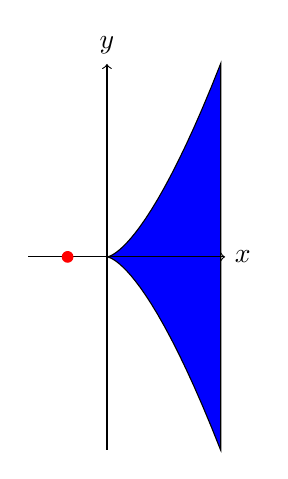
\begin{tikzpicture}[scale=0.5]
\draw[fill=blue, domain=0:1.7, variable=\x] plot({\x*\x}, {\x*\x*\x})
-- (2.89, -4.913) -- plot({(1.7-\x)*(1.7-\x)}, {(1.7-\x)*(1.7-\x)*(\x-1.7)}) 
-- cycle;
\draw[->, black] (-2,0) -- (3,0) node[right] {$x$};
\draw[->, black] (0,-4.9) -- (0,4.9) node[above] {$y$};
\node at (-1,0) [circle,inner sep=1.5pt, fill=red] {};
\end{tikzpicture}
\end{minipage}
\begin{minipage}{0.65\textwidth}
The feasible region is shaded in blue, and the objective function can 
be written as $\|x - [-1,0]\|^2$, i.e. the distance to the point $[-1,0]$
shown as a red dot. Clearly, the minimizer over the feasible region is 
$x^*=[0,0]$.
\end{minipage}
}
\item Find multipliers $\lambda_0$ and $\lambda$ satisfying the 
Fritz John conditions \eqref{2.3.6}.\\
\bluea{Seeing as the only inequality constraint is tight at $x^* = 0$, the 
Fritz John conditions say that there exist $\lambda_0, \lambda\geq 0$ not 
all 0 such that 
\begin{equation*}
\lambda_0 \begin{bmatrix} 2x_1+2 \\ 2x_2 \end{bmatrix}
+ \lambda \begin{bmatrix} -3x_1^2 \\ 2x_2 \end{bmatrix} = 0
\end{equation*}
with $x=0$ plugged in. Indeed, we may take $\lambda_0=0$ and any $\lambda>0$
because the second term is 0.
}
\item Prove there exists no Lagrange multiplier vector for the optimal 
solution. Explain why not. \\
\bluea{
More explicitly plugging in $x^*=0$ to the expression for the gradient 
of the Lagrangian, 
\begin{equation*}
\begin{bmatrix} 2\lambda_0 \\ 0 \end{bmatrix} =0.
\end{equation*}
Therefore, $\lambda_0=0$. Clearly, we cannot have $\lambda_0=1$, as 
required for a Lagrange multiplier vector. This can be explained by 
the fact that the Mangasarian-Fromovitz constraint qualification 
does not hold: for any $d\in\E$, $\ip{\nabla g(x^*), d} = 0$, meaning 
there cannot be $d\in\E$ such that $\ip{\nabla g(x^*), d}<0$.
}
\end{enumerate}
\textbf{3 (Linear independence implies Mangasarian-Fromovitz).} If 
the set of vectors $\{a^1,a^2,\ldots, a^m\}$ in $\E$ is linearly 
independent, prove directly there exists a direction $d\in\E$ satisfying 
$\ip{a^i, d}<0$ for $i=1,2,\ldots, m$. 
\bluea{
\begin{proof}
If the set of vectors is linearly independent, then by definition there 
do not exist $\lambda_1,\ldots,\lambda_m\in\R$ not all 0 such that 
\begin{equation*}
\sum_{i=1}^m \lambda_i a^i = 0,
\end{equation*}
let alone $\lambda_1,\ldots,\lambda_m \geq 0$ summing to 1. Therefore,
the first system of Gordan's theorem is unsolvable. Therefore, the 
second system is, i.e. $\exists d\in\E$ such that $\ip{a^i, d}<0$
 for all $i=1,\ldots, m$.
\end{proof}}
\noindent
\textbf{4.} For each of the following problems, explain why there must 
exist an optimal solution, and find it by using the Karush-Kuhn-Tucker
conditions.
\begin{enumerate}[(a)]
\item 
\begin{equation*}
\begin{aligned}
&\inf && x_1^2 + x_2^2 \\
&\text{subject to}&& -2x_1-x_2 + 19\leq 0 \\
&&& -x_1\leq 0.
\end{aligned}
\end{equation*}
\bluea{
The optimization problem can be rephrased as the distance of the nearest 
point in the intersection of the closed halfspaces $\{x\in\R^2: 
-2x_1-x_2+19\leq 0\}$ and $\{x\in\R^2: -x_1\leq 0\}$ to 0. The 
intersection is convex, closed, and nonempty ($[10,0]$ 
is inside). Therefore,
there exists a unique optimal solution by Exercise 8 of Section 2.1. \\
The KKT conditions (note that they apply here for any feasible point
because $[1,0]$ achieves
a negative product with the gradients of both inequality constraints)
imply for an optimal $x$, there exists $\lambda_1,
\lambda_2\geq 0$ such that 
\begin{equation}
\label{klapklapklap}
2\begin{bmatrix}
x_1 \\ x_2
\end{bmatrix}
- \lambda_1\begin{bmatrix} 2 \\ 1 \end{bmatrix} 
- \lambda_2\begin{bmatrix} 1 \\ 0\end{bmatrix} = 
\begin{bmatrix}
2x_1 - 2\lambda_1 - \lambda_2 \\
2x_2 - \lambda_1
\end{bmatrix} = 
0.
\end{equation}
Furthermore, by complementary slackness, 
\begin{align*}
&\lambda_1(-2x_1 - x_2 + 19) = 0\\
&-\lambda_2 x_1 = 0.
\end{align*}
Notice that $x_1=0$ implies that $x_2 \geq 19$. Furthermore, 
$x_1=0$ implies that $\lambda_1=\lambda_2 = 0$ by the first row of 
\eqref{klapklapklap}. This implies $2x_2=0$, a contradiction. 
Therefore, $\lambda_2=0$ to satisfy complementary slackness. 
By \eqref{klapklapklap} this implies $x_1=\lambda_1$ and 
$\lambda_1=2x_2$, i.e. $x_1=2x_2$. We can't have $\lambda_1=0$, 
because then $x_1=0$ which we ruled out. Therefore, by complementary 
slackness $-2x_1-x_2+19= -5x_2 + 19=0$, i.e. $x_2 = 19/5$ and 
$x_1=38/5$.
}
\item 
\begin{equation*}
\begin{aligned}
&\inf && 5x_1^2 + 6x_2^2 \\
&\text{subject to}&& x_1-4\leq 0\\
&&& 25-x_1^2 - x_2^2 \leq 0.
\end{aligned}
\end{equation*}
\bluea{
Since the inequality constraint functions are continuous, the feasible 
region is closed. Because the objective function has bounded sublevel 
sets, it has a minimizer over the feasible region, i.e. an optimal
solution (note the feasible region is nonempty because $[-5, 0]$ is 
in it). \\
If $\lambda_1,\lambda_2\in\R_+$ compose a Lagrange multiplier vector 
for a feasible point $x$, then 
\begin{equation}
\begin{bmatrix} 10x_1 \\ 12 x_2 \end{bmatrix} + 
\lambda_1\begin{bmatrix} 1 \\ 0 \end{bmatrix} - 
2\lambda_2\begin{bmatrix} x_1 \\ x_2 \end{bmatrix} 
= \begin{bmatrix} 10x_1 + \lambda_1-2\lambda_2x_1 \\ 
12x_2 - 2\lambda_2 x_2 \end{bmatrix} = 0.
\label{234b}
\end{equation}
Furthermore, by complementary slackness, 
\begin{align*}
& \lambda_1(x_1-4) = 0 \\
& \lambda_2(25-x_1^2 - x_2^2) = 0.
\end{align*}
If $\lambda_1=\lambda_2=0$, then by \eqref{234b} implies that 
$[x_1,x_2]=0$, a contradiction because this point is infeasible.
Therefore, at least one constraint is tight. Suppose the first one is, 
i.e. $x_1=4$. Then, the first row of \eqref{234b} implies 
$40+\lambda_1-8\lambda_2=0$. The second equation (note $|x_2| \geq 3$,
because $x_2^2 \geq 25-x_1^2 = 9$) implies $\lambda_2=6$. However,
this implies $\lambda_1 = 8$. We also have $x_1^2 + x_2^2 = 25$ 
because $\lambda_2\neq 0$, and complementary slackness. 
Therefore $x_2 = \pm 3$. Thus, assuming $x_1=4$, the
 only minimizers are $[4, \pm 3]$.\\
 If $x_1 < 4$, then $\lambda_1=0$ by complementary slackness.
This implies $10x_1 - 2\lambda_2x_1 = 0$. If $x_1=0$, then $x_2\neq 0$ 
and thus by $12x_2-2\lambda_2x_2=0$, we have $\lambda_2=6$. Then 
$x_2=\pm 5$. If $x_1\neq 0$, then $\lambda_2 = 5$, implying 
$x_2 =0$, which implies $x_1=-5$. \\
Thus, the only candidate optimal solutions are $[4, \pm 3]$, 
$[0, \pm 5]$, and $[-5, 0]$. They evaluate to 134, 
150, and 125 respectively. Therefore, the optimal solution is 
$[-5,0]$ with objective value 125. (Would have been easier 
to note $5x_1^2 + 6x_2^2 \geq 5(x_1^2+x_2^2) \geq 5(25)=125$.)
}
\end{enumerate}
\textbf{5 (Cauchy-Schwarz and steepest descent).} For a nonzero vector $y$ 
in $\E$, use the Karush-Kuhn-Tucker conditions to solve the problem 
\begin{equation*}
\inf\{\ip{y,x} : \|x\|^2\leq1\}.
\end{equation*}
\bluea{
Note that any nonzero $x$ satisfies the Mangasarian-Fromovitz constraint
qualification condition, and there clearly exists an $x$ for which 
the objective is negative. Therefore, any optimal point must satisfy 
the KKT conditions. \\
The KKT conditions imply that 
\begin{align*}
&y + 2\lambda x = 0 \\
&\lambda(\|x\|^2-1) = 0.
\end{align*}
If $\lambda=0$, then $y=0$, a contradiction since $y$ was assumed nonzero.
Thus, $\|x\|^2=1$ and $y = -2\lambda x$. $\|y\| = 2\lambda\|x\|=2\lambda$
implies $\lambda = \|y\|/2$. This implies $x=-y/\|y\|$. This is thus the 
(unique) optimal solution, with 
objective value $-\|y\|^2$.
}\\
\textbf{6 * (H\"{o}lder's inequality).} For real $p>1$, define $q$ by 
$p^{-1} + q^{-1} =1$, and for $x\in\R^n$ define 
\begin{equation*}
\|x\|_p = \left(\sum_{i=1}^n |x_1|^p\right)^{1/p}.
\end{equation*}
For a nonzero vector $y\in\R^n$, consider the optimization problem 
\begin{equation}
\inf\{\ip{y,x} : \|x\|_p^p\leq 1\}.
\label{2.3.9}
\end{equation}
\begin{enumerate}[(a)]
\item Prove $\frac{d}{du} |u|^p/p = u|u|^{p-2}$ for all real $u$.\\
\bluea{
If $u>0$, then $\frac{d}{du} |u|^p/p = \frac{d}{du} u^p/p = u^{p-1}
= u|u|^{p-2}$.
If $u<0$, then $\frac{d}{du} |u|^p/p = \frac{d}{du}(-u)^p/p = 
-(-u)^{p-1} = u|u|^{p-2}$. \\
To compute the derivative at 0, note $\lim_{u\to 0} |u|^p/pu = 
\lim_{u\to 0} \sgn(u) |u|^{p-1}/p = 0$ since $p>1$.
% To obtain the derivative at 0, let us show the more general fact that 
% if a function $f$ is differentiable on $(\bar x-a, \bar x)$
%  and $(\bar x, \bar x+a)$ for 
% some $a>0, \bar x\in \R$, 
% and $\lim_{x\uparrow\bar x} f'(x) = \lim_{x\downarrow\bar x}
% f'(x) = s$, then $f'(0)= s$.\\
% First let us show $\bar s = 
% \lim_{x\downarrow \bar x} f'(x) = \lim_{x\downarrow
% \bar x} \lim_{t\downarrow 0} \frac{f(\bar x + t)-f(\bar x)}{t}$. This 
% is equivalent to showing that the derivative from the right equals 
% the limit of the derivative from the right. Given $\epsilon > 0$, 
% there exists
}
\item Prove reals $u$ and $v$ satisfy $v=u|u|^{p-2}$ if and only if 
$u=v|v|^{q-2}$. \\
\bluea{
If $u=0$ then clearly $v=0$. Now assume $u >  0$. Thus $v=u^{p-1}$.
Thus $u = v^{1/(p-1)} = v^{q-1}$, since $1/q+1/p=1\implies 
q = p/(p-1) = 1 + 1/(p-1)$. Now if $u < 0$, we have $|u| = |v|^{q-1}$.
Therefore, $u=-|v|^{q-1} = -|v||v|^{q-2} = v|v|^{q-2}$, as 
$v= u|u|^{p-2}$ implies $v<0$.
}
\item Prove problem \eqref{2.3.9} has a nonzero optimal solution.  \\
\bluea{
We have the minimization of a continuous function over a compact set:
the constraint is equivalent to $\|x\|_p\leq 1$,  
$\|\cdot\|_p$ is continuous, and satisfies $\|x\|_\infty > \tau 
\implies \|x\|_p > \tau$. Thus $\|x\|_p\leq \tau \implies 
\|x\| \leq \sqrt{n}\|x\|_{\infty} \leq \sqrt{n}\tau$, i.e. bounded 
sublevel sets. \\
Furthermore, since $y$ is nonzero, we can obtain a negative objective 
by setting one of the entries of $x$ to 1 or $-1$ where $y$ is nonzero.
}
\item Use the Karush-Kuhn-Tucker conditions to find the unique optimal 
solution. \\
\bluea{
The gradient of the constraint is $px|x|^{p-2}$, where operations on 
the vector are done entrywise. If $x$ is nonzero, then clearly we 
can find a $d\in\E$ such that $\ip{px|x|^{p-2}, d} < 0$, thus any 
optimal solution satisfies the KKT conditions. \\
The KKT conditions require $\lambda \geq 0$,
\begin{align*}
& y + \lambda p x|x|^{p-2} = 0\\
& \lambda (\|x\|_p^p -1)=0.
\end{align*}
If $\lambda=0$ then we have $y=0$. Thus, we must have $\|x\|_p^p=1$
and $\lambda\neq 0$. We have $-x|x|^{p-2} = y/\lambda p$. By part (b),
we have $x = -(y/\lambda p)|y/\lambda p|^{q-2}$. 
\begin{equation*}
\|x\|_p = \left\| \bigg|\frac{y}{\lambda p}\bigg|^{q-1}\right\|_p 
= \frac{\||y|^{q-1} \|_p}{ 
\lambda^{q-1}p^{q-1}} = 1
\implies \lambda^{q-1} = \frac{\||y|^{q-1}\|_p}{p^{q-1}}.
\end{equation*}
Use the fact that $q-1 = 1/(p-1)$:
\begin{align*}
\lambda^{1/(p-1)} = \frac{1}{p^{q-1}}\left(\sum_{i=1}^n |y_i|^{p/(p-1)}
\right)^{1/p} = \frac{1}{p^{q-1}}\left(\sum_{i=1}^n |y_i|^q\right)^{1/p}
= \frac{1}{p^{1/(p-1)}}\|y\|_q^{q/p}.
\end{align*}
Use the fact that $(p-1)/p = 1-1/p = 1/q$ to raise both sides to the 
$(p-1)$ power:
\begin{equation*}
\lambda = \frac{\|y\|_q}{p}, \implies 
x = -\frac{y}{\|y\|_q}\bigg|\frac{y}{\|y\|_q}\bigg|^{q-2}
\end{equation*}
}
\item Deduce that any vectors $x$ and $y$ in $\R^n$ satisfy 
$\ip{y,x}\leq \|y\|_q\|x\|_p$. \\
\bluea{
$\sup\ip{y,x} : \|x\|_p \leq 1 = \inf\ip{-y,x}:
\|x\|_p\leq 1$, implying by part 1 that $x=y/\|y\|_q |y/\|y\|_q|^{q-2}$
maximizes $\ip{y,x}$ over $\|x\|_p^p=1$. Then for any nonzero $x$, 
\begin{align*}
&\ip{y,x} = \|x\|_p\ip{y, x/\|x\|_p} \leq \|x\|_p\left\langle 
y, \frac{y}{\|y\|_q}\bigg|\frac{y}{\|y\|_q}\bigg|^{q-2} \right\rangle \\
&\;\;= \|x\|_p\frac{\left(\sum_{i=1}^n |y|^q\right)}{\|y\|_q^{q-1}}
= \|x\|_p\frac{\|y\|_q^q}{\|y\|_q^{q-1}} = \|x\|_p\|y\|_q.
\end{align*}
}
\end{enumerate}
\textbf{7. *} Consider a matrix $A\in\S_{++}^n$ and a real $b>0$.
\begin{enumerate}[(a)]
\item Assuming the problem 
\begin{equation*}
\inf\{-\log\det X : \tr AX\leq b, X\in \S_{++}^n\}
\end{equation*}
has a solution, find it. \\
\bluea{
Let us first compute the gradient of $\tr AX$. Supposing that the 
gradient of a function $f(X)$ exists, the directional derivative
 of $f(AX)$ is 
\begin{equation*}
\lim_{t\downarrow 0} \frac{f(A(X+tY)) - f(AX)}{t} 
= f'(AX; AY) = \ip{(\nabla f)(AX), AY} = \ip{A(\nabla f)(AX), Y},
\end{equation*}
using the fact that $A$ is symmetric. Therefore, $\nabla f(AX) = 
A(\nabla f)(AX)$. Thus, the gradient of the constraint is $A$. This 
implies that an optimal solution must satisfy the KKT conditions, because 
clearly there exists $B\in\S^n$ such that $\ip{A,B} < 0$. The gradient 
of the objective is $-X^{-1}$. Now the KKT conditions state there 
exists $\lambda \geq 0$ such that 
\begin{align*}
&-X^{-1} + \lambda A = 0 \\
&\lambda (\tr AX - b) = 0.
\end{align*}
If $\lambda=0$, we obtain a contradiction as $X^{-1}$ cannot equal 0. 
Therefore, $\tr AX - b =0 $. Then the first equation, after 
right multiplying by $X$ and taking the trace, implies $\lambda = n/b$.
Thus $X = \frac{b}{n} A^{-1}$.
}
\item Repeat using the objective function $\tr X^{-1}$. \\
\bluea{
Now the KKT conditions state 
\begin{align*}
& - X^{-2} + \lambda A = 0 \\
& \lambda (\tr AX - b ) = 0.
\end{align*}
Again, we cannot have $\lambda = 0$ because $-X^{-2}\neq 0$. We have 
$X^{-2} = \lambda A$, i.e. $X^2 = A^{-1}/\lambda \implies X = 
\sqrt{A^{-1}/\lambda}$. Plugging this into $\tr AX = b$, we get 
$\lambda^{-1/2} \tr \sqrt{A} = b \implies \lambda = (\tr\sqrt{A}/b)^2$.
Plugging this into $X=\sqrt{A^{-1}/\lambda}$, we get 
$X = \frac{b \sqrt{A^{-1}}}{\tr\sqrt{A}}$.
}
\item Prove the problems in parts (a) and (b) have optimal solutions.
(Hint: Section 1.2, Exercise 14.) \\
\bluea{
Section 1.2, Exercise 14 says that for any positive definite matrix $C$, 
the function $\ip{C, X} - \log\det X$ has compact sublevel sets. 
Notice that $\tr AX \leq b$ implies $\ip{A,X} - \log\det X \leq 
b-\log\det X$. We have the feasible point $X = bI/n\tr A$. 
Therefore, we can restrict the domain of the infimum to 
$\{X:\tr AX \leq b\} \cap \{X: \ip{A,X}-\log\det X \leq b - 
\log\det (bI/n\tr A)\}$. The first set is closed (in fact, compact) 
due to $\tr AX$ being continuous and the second set 
is compact, so the domain is compact, implying the existence of a 
minimizer. \\
For (b), note that $\tr X^{-1}\leq \alpha$ implies that the minimum 
eigenvalue of $X,\; \lambda_n(X)$
 is $\geq 1/\alpha$. 
Denoting $a>0$ as the minimum eigenvalue of $A$, 
$\tr AX \leq b$ implies $\lambda_1(X)\leq b/a$. Therefore, 
$\{X : \tr X^{-1}\leq \alpha\} \cap \{X: \tr AX \leq b\}$
is compact, because it is the intersection of two sets that are closed 
in $\S_{++}^n$, and the intersection is contained in $\inter \S_{++}^n$
and bounded because $\frac{1}{\alpha}\leq \lambda_n(X) \leq \lambda_1(
X) \leq \frac{b}{a}$.
}
\end{enumerate}
\textbf{8 ** (Minimum volume ellipsoid).} 
\begin{enumerate}[(a)]
\item For a point $y\in\R^n$ and the function $g:\S^n\to\R$ defined by 
$g(X)=\|Xy\|^2$, prove $\nabla g(X) = Xyy^\top + yy^\top X$ for all 
matrices $X\in\S^n$. \\
\bluea{
\begin{align*}
&\lim_{t\downarrow 0} \frac{\|(X+tY)y\|^2 - \|Xy\|^2}{t} 
= \lim_{t\downarrow 0} \frac{y^\top (X+tY)^2 y - y X^2 y}{t} \\
&\;
= \lim_{t\downarrow 0} \frac{ y^\top X^2 y + t y^\top XY y + t y^\top YX
y + t^2 y^\top Y y - y X^2 y }{t}\\
&\; = \tr y^\top XY y + \tr y^\top YX y = \tr yy^\top X Y + \tr Xyy^\top Y
= \ip{yy^\top X + Xyy^\top, Y},
\end{align*}
after which it follows that $\nabla g(X) = Xyy^\top + yy^\top X$.
}
\item Consider a set $\{y^1,y^2,\ldots,y^m\}\subset\R^n$. Prove this set 
spans $\R^n$ if and only if the matrix $\sum_i y^i (y^i)^\top$ is 
positive definite. \\
\bluea{
If it does not span $\R^n$, then there exists nonzero
 $x\in\R^n$ orthogonal 
to $y^1,\ldots, y^m$. Then $x^\top\left(\sum_i y^i(y^i)^\top\right)x = 0$.
\\
If it does span $\R^n$, then suppose some $x\in\R^n$ satisfies 
$x^\top\left(\sum_i y^i (y^i)^\top \right) x = 0$. Since each 
$x^\top y^i (y^i)^\top x = (x^\top y^i)^2 \geq 0$, this implies that 
each term equals 0. In other words, $x$ is orthogonal to 
$\{y^1,\ldots, y^m\}$. But this contradicts $\{y^1,\ldots, y^m\}$
spanning $\R^n$. (If $x=\sum_i c_iy^i$, then $\|x\|^2 = 
x^\top \sum_i c_iy^i = 0$, a contradiction.)
}
\item Now suppose the vectors $y^1,\ldots,y^m$ span $\R^n$.
 Prove the problem 
\begin{equation*}
\begin{aligned}
&\inf && -\log\det X &&\\
&\text{subject to} && \|Xy^i\|^2 - 1\leq 0 && \forall i=1,\ldots, m\\
&&& X\in\S_{++}^n
\end{aligned}
\end{equation*}
has an optimal solution. (Hint: Use part (b) and Section 1.2, Exercise 
14.) \\
\bluea{
Since $\tr (\sum_i y^i (y^i)^\top) X - \log\det X$ has compact level 
sets, and we know that $\tr (\sum_i y^i (y^i)^\top)X \leq n$ from
the constraints, we can take the objective value at some feasible $X$,
add it to $n$, and know that the optimal $X^*$ is contained in the 
compact level set corresponding to that objective value. After 
intersecting this level set with the closed sets $\{X: \|Xy^i\|^2 \leq 1\}
$, we obtain a compact subset of the feasible region containing $X^*$.
}
\item Now suppose $\bar X$ is an optimal solution for the problem in 
part (c). (In this case the set $\{y\in\R^n : \|\bar Xy\|\leq 1\}$ is a 
minimum volume ellipsoid centered at the origin containing the vectors 
$y^1,y^2,\ldots, y^m.$)
Show the Mangasarian-Fromovitz constraint qualification holds at $\bar X$ 
by considering the direction $d=-\bar X$. \\
\bluea{
We need to show that for every $i=1,\ldots, m,\; \ip{\bar X yy^\top 
+ yy^\top \bar X, -\bar X} < 0$. Evaluating the inner product gives 
$-2y^\top \bar X^2 y < 0$.
}
\item Write down the Karush-Kuhn-Tucker conditions that $\bar X$ must 
satisfy.  \\
\bluea{
The KKT conditions are: 
\begin{align*}
&-\bar X^{-1} + \sum_{i=1}^m \bar Xy^i(y^i)^\top + \bar y^i(y^i)^\top 
X = 0\\
& \forall i\in [m],\; \lambda_i(\|Xy^i\|^2-1)= 0.
\end{align*}
}
\item When $\{y^1, y^2, \ldots, y^m\}$ is the standard basis of $\R^n$, 
the optimal solution of the problem in part (c) is $\bar X=I$. Find the 
corresponding Lagrange multiplier vector. \\
\bluea{
We have 
\begin{equation*}
-I + 2\sum_{i=1}^n \lambda_i e_ie_i^\top 
= \sum_{i=1}^n (2\lambda_i-1) e_ie_i^\top = 0
\end{equation*}
implying $\lambda_i = \frac{1}{2}$ for each $i=1,\ldots, n$. Note 
each constraint $\|Xy^i\| = \|e_i\|^2 = 1$ is tight.
}
\end{enumerate}
\end{document}
